\documentclass[11pt,a4paper]{article}
\usepackage[utf8]{inputenc}
\usepackage{amsmath}
\usepackage{amsfonts}
\usepackage{amssymb}
\usepackage{graphicx}
\usepackage[french]{babel}
\usepackage{pgfornament}
\usepackage{braket}
\usepackage{tikz}
\usetikzlibrary{calc}
\usepackage{fancyhdr}
\pagestyle{fancy}



\usepackage[left=2cm,right=2cm,top=2cm,bottom=3cm]{geometry}

\author{Alain Delaët-Tixeuil \and André Kalouguine}
\title{Systemes quantiques uniques, décohérence et trajectoires quantiques.}
\date{8 mai 2018}

\renewcommand{\thesection}{\Alph{section}}
\renewcommand{\thesubsection}{\thesection.\roman{subsection}}
\newcommand{\q}{q\hspace{-0.5ex}u}
\renewcommand{\S}{\ensuremath{\mathfrak{S}}}
\newcommand{\E}{\ensuremath{\mathfrak{E}}}
\newenvironment{qd}[1]{\par\vspace{2em}%
	\noindent\textbf{Définition: } \texttt{#1}: \\
	\begin{tikzpicture}
		\node[text width=\linewidth-1cm] (txt) at (3,0) \bgroup
}{\egroup;
		\node[rotate=-90](a) at ($(txt.west)+(-0.75,-0.1)$) {\pgfornament[width=3cm]{85}};
		\end{tikzpicture}%
\\
}
\begin{document}
	\maketitle
	\begin{abstract}
		On étudie ici le comportement des systèmes quantiques simples lors de la présence d'une source de décohérence. Une méthode principalement numérique est utilisée. Deux points de vue de l'apparition de la décohérence sont présentés: l'équation de Lindblad avec des opérateurs de saut et les trajectoires quantiques en présence de la mesure faible et forte par l'environnement.
	\end{abstract}
	\section{Systèmes quantiques uniques}
	Certains systèmes quantiques présentent un nombre limité de degrés de liberté et peuvent être étudiés d'un point de vue individuel et non pas comme un mélange statistique. Parmi ces systèmes; \q bits et oscillateurs harmoniques.
	L'évolution de ces systèmes est régie par l'équation de Schrödinger:
	\begin{equation}
			i\hbar \frac{\textrm{d}\rho}{\textrm{dt}}=\left[\mathcal{H},\rho\right]
	\end{equation}
	ou $\rho$ est la matrice de densité. Lorsque l'on reste dans le cas des systèmes purs, la matrice de densité est juste $\rho=\ket{\psi}\bra{\psi}$ ou $\psi$ est la fonction d'onde.
	\subsection{Systèmes a deux niveaux (\q bits)}
	Certains systèmes quantiques présentent une structure a deux états séparés. Prenons par exemple une molécule d'ammoniac:
	\begin{figure}[!ht]
		\centering
		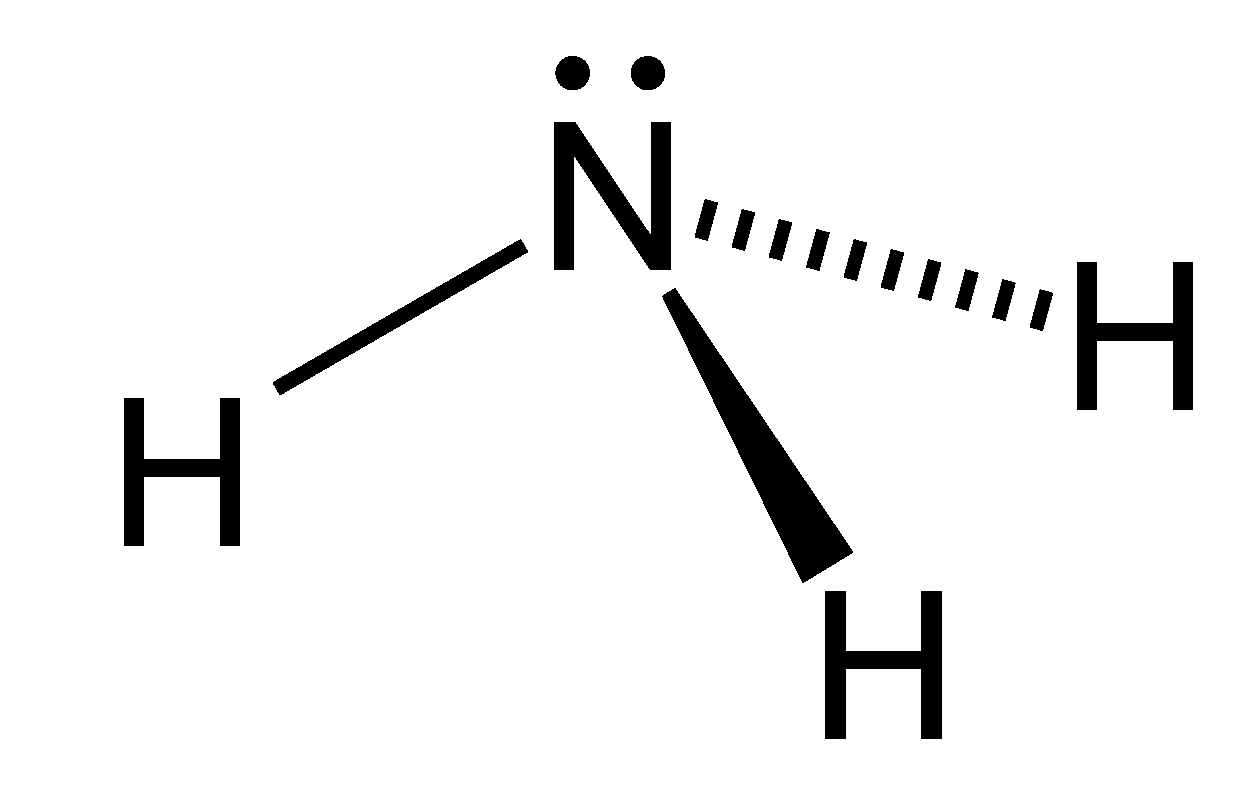
\includegraphics[width=0.4\linewidth]{ammonia}
		\caption{Structure de l'ammoniac.}
		\label{fig:ammonia}
	\end{figure}
	L'atome d'azote se trouve a cette position puisque c'est un minimum d'énergie potentielle local. Vu la symétrie de la molécule, son image miroir a la même énergie. L'atome d'azote a donc deux positions stables des deux cotés du plan des hydrogènes. Si l'on étudie l'atome d'azote uniquement, on peut le considérer comme une particule libre pouvant bouger sur un axe 1D dans un potentiel symétrique.
		
	\begin{figure}[!ht]
		\centering
		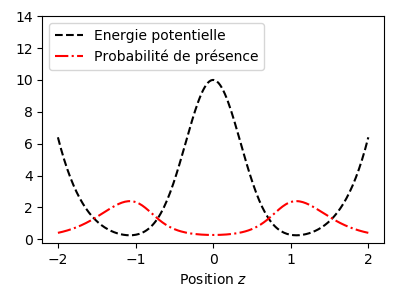
\includegraphics[width=4in]{DbleWell}
		\caption{Exemple de double puit de potentiel.}
		\label{fig:dblewell}
	\end{figure}
	
	\noindent On identifie deux états correspondants a la majorité de la fonction d'onde se trouvant d'un coté ou de l'autre de la barrière. On va noter ces deux états $\ket{0}$ et $\ket{1}$. On les construit de manière a avoir $\braket{0|1}=0$.
	
	L'hamiltonien de ce système doit être hermitien, donc sa forme la plus générale est:
	\[
		\mathcal{H}=\left[\begin{matrix}
		\epsilon_0 & \delta\textrm{e}^{i\varphi}\\
		\delta\textrm{e}^{-i\varphi} & \epsilon_1
		\end{matrix}\right]
	\]
	Cet hamiltonien se diagonalise en
	\[
	\mathcal{H}=\left[\begin{matrix}
	E_+ & 0\\
	0 & E_-
	\end{matrix}\right]=
	\left[\begin{matrix}
	\epsilon+\sqrt{\Delta\epsilon^2+\delta^2} & 0\\
	0 & \epsilon-	\sqrt{\Delta\epsilon^2+\delta^2}
	\end{matrix}\right]
	\]
	ou $\displaystyle \epsilon=\frac{\epsilon_0+\epsilon_1}{2}$ et $\displaystyle \Delta\epsilon=\frac{\epsilon_1-\epsilon_0}{2}$.
	
	\noindent Les vecteurs propres de cet hamiltonien sont\\ $\ket{+}=
	\left|\begin{matrix}
	\sqrt{\frac{E_+-\epsilon_1}{E_+-E_-}}\\
	\sqrt{\frac{E_+-\epsilon_0}{E_+-E_-}}\textrm{e}^{i\varphi}
	\end{matrix}\right.$ 
	et $\ket{-}=
	\left|\begin{matrix}
	\sqrt{\frac{E_--\epsilon_1}{E_--E_+}}\\
	\sqrt{\frac{E_--\epsilon_0}{E_--E_+}}\textrm{e}^{-i\varphi}
	\end{matrix}\right.$.
	
	\vspace{1em}\noindent Le système placé dans un état $\ket{\psi(0)}=\alpha\ket{+}+\beta\ket{-}$ va donc évoluer ainsi: $\ket{\psi(t)}=\alpha\textrm{e}^{iE_+/\hbar}\ket{+}+\beta\textrm{e}^{iE_-/\hbar}\ket{-}$. Donc sa représentation sur la sphère de Bloch va tourner. 
	Ci joint, un exemple (on utilise partout $\hbar=1$) avec $\mathcal{H}=\hbar\omega\sigma_z$: (Fig. \ref{fig:qubit})
	\begin{figure}
		\centering
		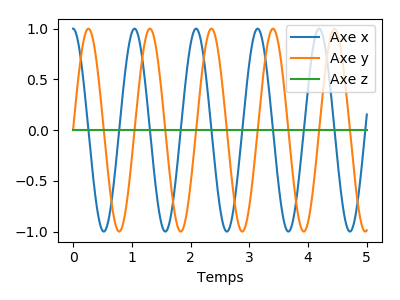
\includegraphics[width=0.7\linewidth]{Qubit}
		\caption{Q\hspace{-0.5ex}ubit avec $\omega=3$ et $\ket{\psi_0}=\frac{\ket{0}+\ket{1}}{\sqrt{2}}$}
	\label{fig:qubit}
	\end{figure}
	
	
	
	\subsection{Oscillateur harmonique}
	Un autre système simple est l'oscillateur harmonique qui correspond a un potentiel parabolique:
	\[
	\mathcal{H}=\frac{p^2}{2m}+\frac 12 m\omega^2x^2=\hbar\omega \left(a^{\dag} a+\frac 12\right)
	\]\\
	ou l'on a $\displaystyle a=\sqrt{\frac{m\omega}{2\hbar}}\left(x+\frac{i}{m\omega}p\right)$\\
	Posons $N=a^{\dag} a$. Soit $\ket{\psi}$ un eigenvecteur de $\mathcal{H}$ et donc de $N$: $N\ket{\psi}=\lambda\ket{\psi}$.
	Alors $Na^{\dag}\ket{\psi}=([N,a^{\dag}]+a^{\dag}N)\ket{\psi}=a^{\dag}(N+1)\ket{\psi}=(\lambda+1)a^{\dag}\ket{\psi}$. De plus, on a $N$ hermitien, donc $\lambda\geqslant0$. Donc $\mathbb{N}$ est l'ensemble des eigenvaleurs de $N$ et on pose l'état associé a $\lambda=n$ comme $\ket{n}$. Ces états sont appelés les états de Fock. et ce sont les états stationnaires de l'oscillateur harmonique.
	\begin{qd}{Pseudo-probabilité de Wigner}
		A l'instar d'une particule classique dont l'état est entièrement donné par ses coordonnées dans l'espace de phase, un état quantique est entièrement défini par une distribution de \emph{pseudo-probabilité} sur l'espace $\{x,p\}$ appelée distribution de Wigner.
		$
			P(x,p)=\frac{1}{\pi\hbar}\int\braket{x+y|\rho|x-y}\textrm{e}^{-2i\pi y / \hbar}\textrm{dy}
		$
		ou $\rho$ est la matrice de densité.
		La négativité de la fonction indique que l'état n'a pas d'analogue classique.
	\end{qd}

	On peut représenter quelques états de Fock: (Fig. \ref{fig:fock})
	\begin{figure}
		\centering
		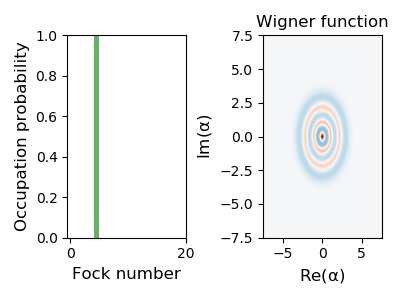
\includegraphics[width=0.7\linewidth]{Fock}
		\caption{État de Fock avec $n=5$ photons. Distribution de Wigner a droite.}
		\label{fig:fock}
	\end{figure}
	
	
	On observe que tous les états de Fock sauf l'état du vide sont strictement quantiques.
	Bien évidemment les états de Fock sont stationnaires. Mais une superposition de deux états de Fock permet de visualiser les oscillations de Rabi vues dans le cadre du \q bit. Cette fois-ci on peut directement représenter la probabilité de de détection d'un photon en fonction de $x$. On observe une évolution périodique donnant lieu a une espérance de $x$ oscillante (Fig. \ref{fig:2fock_evol_val})
	
	\begin{figure}
		\centering
		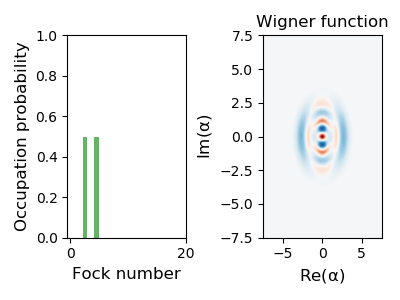
\includegraphics[width=0.7\linewidth]{2Fock}
		\caption{Superposition de deux états de Fock. Instant initial.}
		\label{fig:2fock}
	\end{figure}

	\begin{figure}
		\centering
		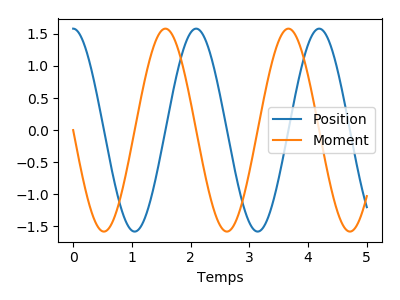
\includegraphics[width=0.7\linewidth]{2Fock_evol_val}
		\caption{Évolution de l'espérance du moment et de la position pour une superposition de 2 états de Fock.}
		\label{fig:2fock_evol_val}
	\end{figure}
		
	
	Un état qui a un analogue classique est l'état cohérent, eigenvecteur de $a$. 
	Sa décomposition dans la base de Fock est une distribution poissonnienne de paramètre $\alpha$. L'espérance du nombre de photons est $|\alpha|^2$: (Fig. \ref{fig:coherent_distr})
	\begin{figure}
		\centering
		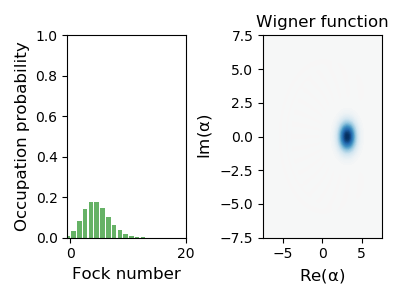
\includegraphics[width=0.7\linewidth]{Coherent_distr}
		\caption{Une distribution cohérente avec $\alpha=\sqrt{10}$.}
		\label{fig:coherent_distr}
	\end{figure}
	
	Cet état a un comportement classique, il tourne. On peut estimer aussi la position et le moment moyens, et le comportement est similaire au comportement classique et le paquet oscille: (Fig. \ref{fig:coherent_evol})
	\begin{figure}
		\centering
		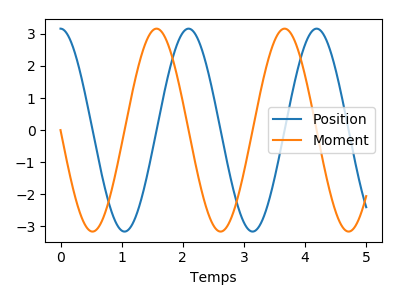
\includegraphics[width=0.7\linewidth]{Coherent_evol_val}
		\caption{Évolution d'un état cohérent a 10 photons en moyenne.}
		\label{fig:coherent_evol}
	\end{figure}
	
	Un comportement purement quantique peut être observé lorsque il y superposition de deux états cohérents. On a alors apparition de franges négatives sur la distribution de Wigner, signe de la nature quantique.
	Si on étudie la probabilité de présence selon $x$, on observe ces franges lorsque les deux paquets cohérents se retrouvent a $x$ proche de 0.
	
	\begin{figure}
		\centering
		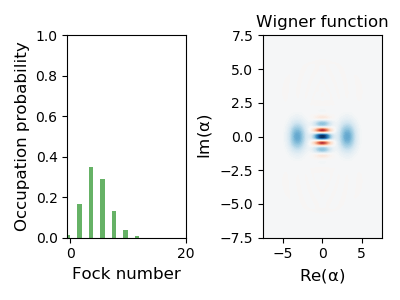
\includegraphics[width=0.7\linewidth]{Sum_coherent}
		\caption{Superpostion de deux états cohérents avec $\alpha_1=-\alpha_2$ a l'instant initial. Toute la figure tourne.}
		\label{fig:sum_coherent}
	\end{figure}
	
	\section{Décohérence}
	Lorsque le système quantique n'est pas parfaitement isolé de l'environnement, il y a perte de cohérence et le système devient un mélange statistique classique d'états purs. On parle alors de décohérence.
	Les systèmes quantiques simple que l'on a étudié auparavant permettent de modéliser cela en utilisant des opérateurs de "saut" (\emph{jump operators}).
	
	On peut alors écrire une équation différentielle sur $\rho$, la matrice de densité du système. Pour rappel, lorsque le système n'interagit pas avec l'environnement, on a l'équation de Schrödinger:
	\[
	i\hbar \frac{\textrm{d}\rho}{\textrm{dt}}=\left[\mathcal{H},\rho\right]
	\]
	
	On considère l'évolution d'une matrice de densité de probabilité entre $t$ et $t+\tau$. C'est le résultat d'application d'un opérateur linéaire qui conserve l'herméticité, la trace, la positivité de la matrice de densité. On montre que cet opérateur $\mathcal{L_{\tau}}$ peut s'écrire comme $\mathcal{L_{\tau}}=\sum_i L_i(\tau)\rho(t)L_i(\tau)^{\dag})$ ou les $L_i$ sont les opérateurs de Kraus, ou opérateurs de saut
	
	
	On trouve après simplification que pour un système en contact avec l'environnement on a:
	\begin{equation}
	\frac{\textrm{d}\rho}{\textrm{dt}}=-\frac{i}{\hbar}\left[\mathcal{H},\rho\right]+\sum_{\mu}\left(
	L_{\mu}\rho L_{\mu}^{\dag}-\frac 12 L_{\mu}^{\dag}L_{\mu}\rho -\frac 12 \rho L_{\mu}^{\dag}L_{\mu}
	\right)
	\end{equation}
	C'est l'équation de Lindblad.
	L'équation décrit l'interaction d'un système quantique avec un modèle simplifié de l'environnement qui a une dimension finie, specifiquement celle du nombre d'opérateurs de Kraus. Entre les moments de temps $t$ et $t+\tau$, il y a une certaine probabilité que le système va passer de l'état $\ket{\psi}$ à l'état $L_{\mu}\ket{\psi}$, ce qui modélise l'interaction avec l'environnement.
	
	On peut étudier grâce à QuTiP l'évolution des systèmes quantiques simples et l'apparition de la décohérence.
	
	\subsection{Décohérence d'un \q bit}
	Considŕons un \q bit dans un bain thermique. Le \q bit peut sous l'influence de l'environnement perdre de l'énergie. Ainsi l'opérateur $L=\left[\begin{matrix}
	1&1\\0&0
	\end{matrix}\right]$ fait passer le systeme dans l'état $\ket{0}$. On observe alors ces mêmes oscillations de Rabi mais cette fois ci atténuées. On voit aussi que le \q bit tend vers l'état $\ket{0}$: (Fig. \ref{fig:qubit_deco1})
	\begin{figure}
		\centering
		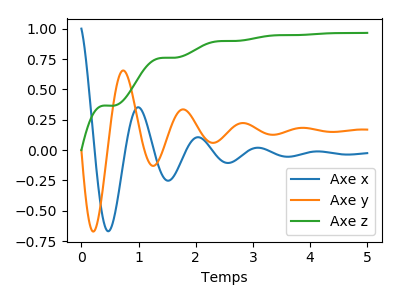
\includegraphics[width=0.7\linewidth]{Qubit_deco1}
		\caption{Décohérence d'un \q bit lorsque il peut être collapsé dans son état $\ket{0}$}
		\label{fig:qubit_deco1}
	\end{figure}
	
	Il y a pour un \q bit un autre canal de décohérence important: la perte de phase. On peut le modéliser par un opérateur de saut qui va rajouter une déphasage de $\pi$ entre les deux composantes du \q bit. On observe naturellement pas de perte d'énergie. Plutot, le \q bit tend vers le point au centre de la sphère de Bloch, qui correspond a un mélange statistique équitable de $\ket{0}$ et $\ket{1}$: (Fig. \ref{fig:qubit_deco2})
	\begin{figure}
		\centering
		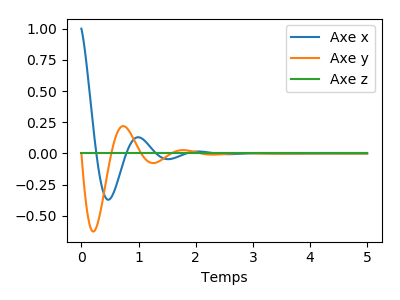
\includegraphics[width=0.7\linewidth]{Qubit_deco2}
		\caption{Décohérence d'un \q bit lorsque il y a sauts de phase mesurés par l'environnement.}
		\label{fig:qubit_deco2}
	\end{figure}
	
	
	
	\subsection{Décohérence d'un oscillateur harmonique}
	Pour un oscillateur harmonique, c'est assez naturel que lorsque il est dans un bain thermique, il puisse perdre des photons ou en gagner, et les deux taux vont dépendre de la température du bain.
	On introduit donc deux opérateurs de saut: $L_0=\sqrt{\Gamma_0}\cdot a$ (perte de photon a un taux $\Gamma_0$); et $L_1=\sqrt{\Gamma_1}\cdot a^{\dag}$ (création d'un photon a un taux $\Gamma_1$)
	
	Étudions l'effet de ce couplage sur certains états.
	
	Si l'on prend un état de Fock, on observe bien la chose logique: il y a décroissance exponentielle du nombre de photons:(Fig. \ref{fig:Fock_deco_conti})
	\begin{figure}
		\centering
		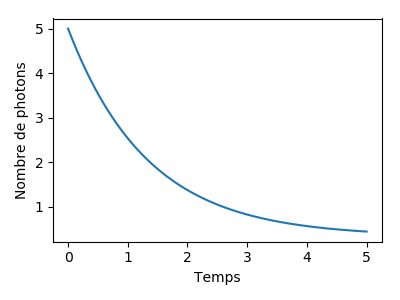
\includegraphics[width=0.7\linewidth]{Fock_deco_conti}
		\caption{Perte de photons dans un oscillateur dans un état de Fock.}
		\label{fig:Fock_deco_conti}
	\end{figure}
	
	On peut regarder un état cohérent, la situation sera la même, malgré le fait que l'état cohérent est eigenvecteur de $a$. Cela est du au fait que QuTiP modélise aussi la mesure faible qu'on effectue du nombre de photons. Malgré le fait que c'est une mesure faible, elle est faite en même temps que la simulation (la faire après, n'a pas de sens physique) et l'influence donc. Ainsi, lorsque l'on ne mesure pas de photons dans l'oscillateur, ce qui arrive avec une certaine probabilité, on mets a jour notre connaissance du système. La probabilité qu'il n'y ait pas de photons chute alors.
	
	Un cas plus intéressant a étudier est celui d'une superposition d'états cohérents.  Pour rappel, si il n'y a pas de décohérence, la distribution de Wigner présente des franges purement quantiques. On observe une disparition très rapide de ces franges lorsque l'oscillateur peut perdre des photons: (Fig. \ref{fig:Coh_sum_deco})
	\begin{figure}
		\centering
		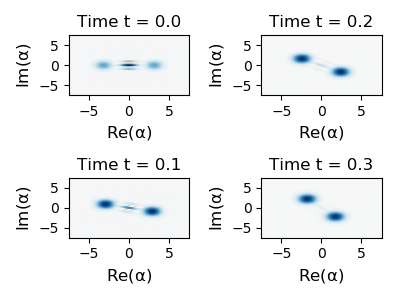
\includegraphics[width=0.7\linewidth]{Coh_sum_deco}
		\caption{Disparition des franges. Les quatre distributions présentent 4 instants de temps différents.}
		\label{fig:Coh_sum_deco}
	\end{figure}

	On peut montrer que il y a perte d'information en regardant l'entropie de Von Neumann du système (voir Fig.	\ref{fig:Entropy} ). On voit au début une  augmentation  de l'entropie due a la décohérence et disparition du système. Puis il y a décroissance de l'entropie, ce qui correspond probablement au fait que l'oscillateur arrive a l'état du vide.
	

	\begin{figure}
		\centering
		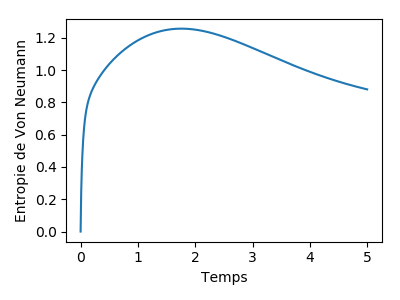
\includegraphics[width=0.7\linewidth]{Entropy}
		\caption{Augmentation de l'entropie du système lorsque il y a interaction avec l'environnement.}
		\label{fig:Entropy}
	\end{figure}
	
	\section{Trajéctoires uniques}
	
	Un moyen de voir la décohérence est d'effectuer plusieurs fois la même expérience avec des mesures effectuées par l'environnement. Chacune de ces mesures conduit a un collapse de l'état dans un état propre de l'opérateur de mesure.
	En moyennant sur plusieurs expériences, on est sensé retrouver la matrice de densité obtenue avec Lindblad.
	
	Pour cela dans QuTiP, on utilise le solveur de Monte-Carlo.
	
	\subsection{Décohérence d'un \q bit}
	Lorsque on utilise l'opérateur de saut $L=\left[\begin{matrix}
	1&1\\0&0
	\end{matrix}\right]$, on observe exactement ce a quoi on s'attend: le \q bit collapse a un moment aléatoire dans l'état $\ket{0}$:  (Fig. \ref{fig:u_qubit_deco2})
	\begin{figure}
		\centering
		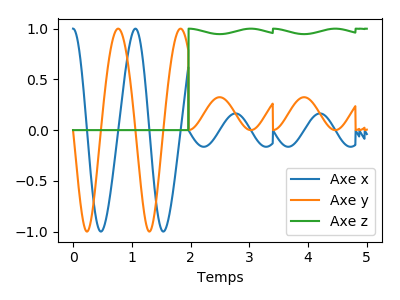
\includegraphics[width=0.7\linewidth]{U_Qubit_deco1}
		\caption{Mesure stochastique effectuée a l'instant $t\approx 2$}
		\label{fig:u_qubit_deco2}
	\end{figure}
	Les oscillations après le collapse sont dues aux erreurs de calcul.
	Si l'on moyenne cela sur une centaine de trajectoires, on se rapproche de la solution donnée par Lindblad: (Fig. \ref{fig:u_qubit_deco1_100})
	\begin{figure}
		\centering
		\includegraphics[width=0.7\linewidth]{U_qubit_deco1_100}
		\caption{Moyenne sur 100 expériences. A comparer avec (Fig. \ref{fig:qubit_deco1})}
		\label{fig:u_qubit_deco1_100}
	\end{figure}

	De même, lorsque il en est a la perte de phase. Représentons juste la moyenne sur 100 expériences:(Fig. \ref{fig:u_qubit_deco2_100})
	\begin{figure}
		\centering
		\includegraphics[width=0.7\linewidth]{U_qubit_deco2_100}
		\caption{Moyenne sur 100 expériences. A comparer avec (Fig. \ref{fig:qubit_deco2})}
		\label{fig:u_qubit_deco2_100}
	\end{figure}


	\subsection{Décohérence d'un oscillateur harmonique}
	
	On peut faire de même avec un oscillateur harmonique. Plaçons nous d'abord dans un état de Fock. Une seule réalisation de l'expérience lorsque deux opérateurs de sauts: $a$ et $a^{\dagger}$ est exactement ce a quoi l'on s'attendrait: l'oscillateur reste dans des états de Fock, mais le nombre de photons change stochastiquement: (Fig. \ref{fig:U_Fock_deco_1})
	\begin{figure}
		\centering
		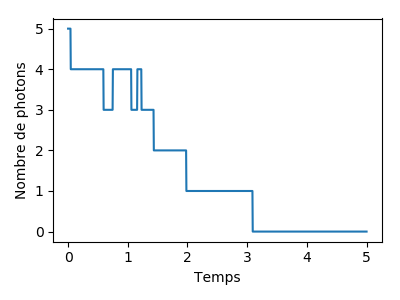
\includegraphics[width=0.7\linewidth]{U_Fock_deco_1}
		\caption{On part de 5 photons, on observe une trajectoire unique.}
		\label{fig:U_Fock_deco_1}
	\end{figure}

	Lorsque on effectue plusieurs mesures, on retrouve bien la décroissance exponentielle.
	
	Lorsque l'on se place dans un état cohérent, on observe une décroissance exponentielle entre les saut du nombre de photons. Comme précédemment, cela résulte du fait que les mesures faibles influencent quand même le système.
	
\end{document}